\documentclass[../SimBALink.tex]{subfiles}
\begin{document}

\section{Motor model performance}
	xxx
	\subsection{Calibration}
		dafsd
		
		\subsubsection{Efficiency model}
			The motor efficiency model was derived from an efficiency plot provided by the manufacturer. 
			
			\begin{figure}[h]
				\centering
				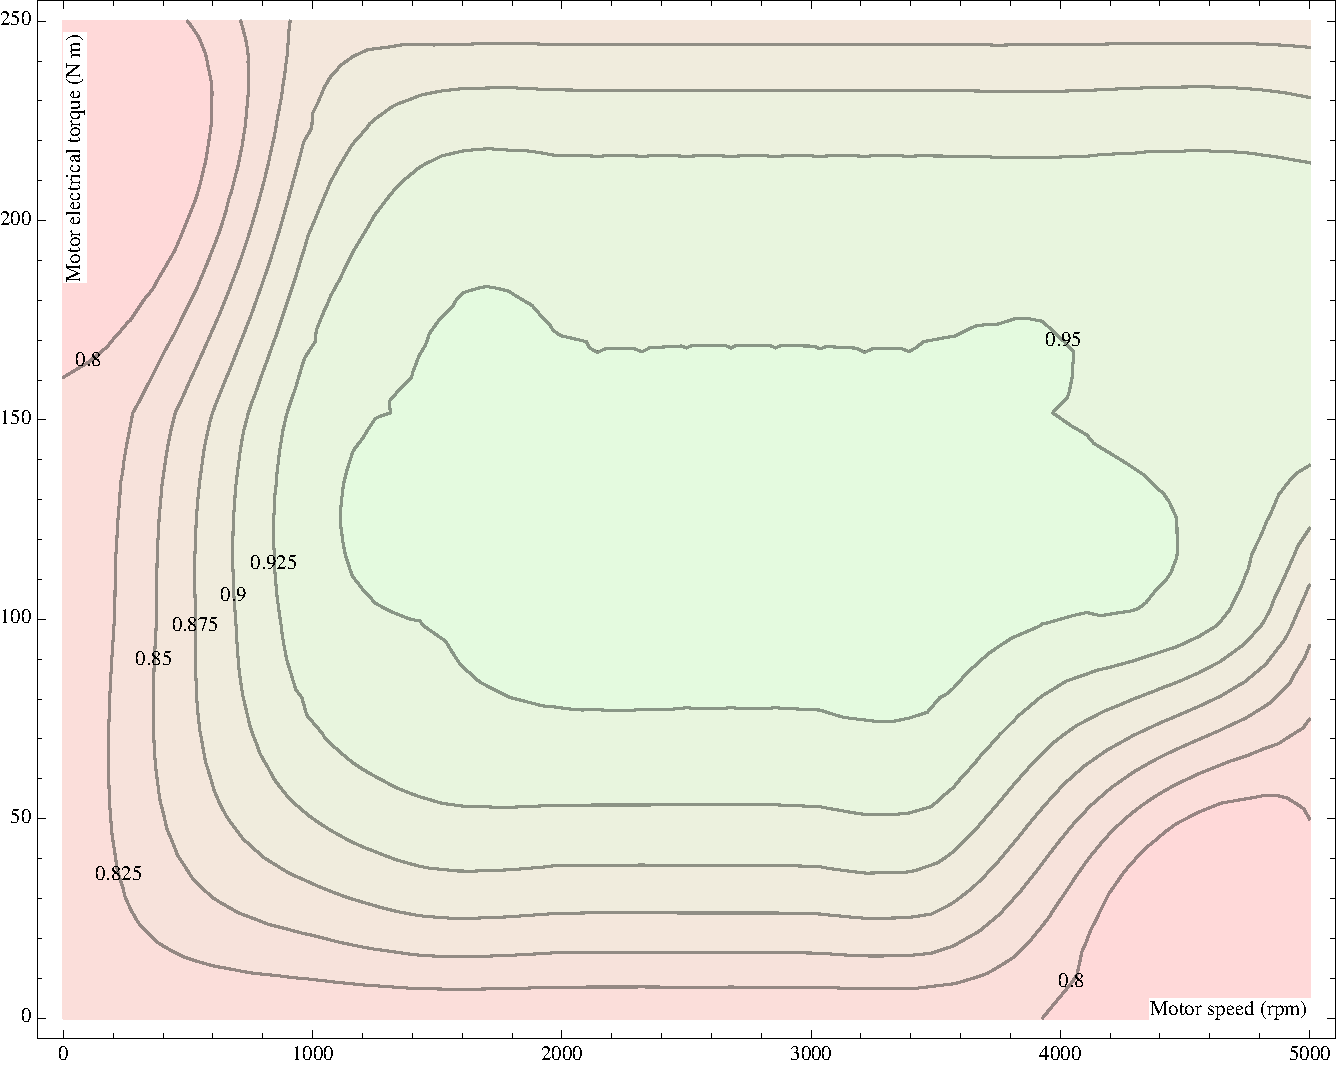
\includegraphics[width=4in]{../Model/Powertrain/Motor/Documentation/Figures/EMRAX_228HV_efficiency}
				\caption{Enstroj EMRAX 228HV - motor efficiency over operating range.}
			\end{figure}
			\FloatBarrier
			
			The efficiency plot is based on variables which are convenient to measure using an engine dynamometer and a power inverter. In future testing, the efficiency function will be derived from steady-state experimental data.
			
		\subsubsection{Equivalent-circuit parameters}
			The motor manufacturer specifies values for $L_d$, $L_q$, and $R$. Since the model performance was good without additional calibration of these values, they were used unchanged.
			
			The only equivalent-circuit parameter that was calibrated in the model was $\phi$, the permanent-magnet flux linkage.
						
			\begin{table}
				\centering
				\caption{Calibrated parameters in motor model}
				\label{table:motor_calibrated_parameters}
				\begin{tabular}{c | l | c | c}
					Symbol		&	Parameter			&	Initial guess value	&	Calibrated value	\\
					\hline
					$\phi$		&	Motor flux linkage		&	1 V rad/sec	 	&	24.5 m$\Omega$
				\end{tabular}
			\end{table}
			
			The capacity parameter was included as a calibrated parameter because initial tests with the model displayed what appeared to be a scaling error in the model's open-circuit voltage term.
			
	\subsection{Model validation and quality of fit}
		insert insightful content here
		
		
\end{document}